\documentclass[12pt]{article}
\usepackage[english]{babel}
\usepackage[utf8]{inputenc}
\usepackage{parskip}
\usepackage[usenames,dvipsnames]{xcolor}
\usepackage[pdftex]{graphicx}
\usepackage{wrapfig}
\usepackage{hyperref}
\usepackage{tabularx}
\usepackage{pdflscape}
\hypersetup{colorlinks=true, urlcolor=magenta, linkcolor=orange, pdfauthor=Alejandro López Espinosa, pdftitle=título}
\usepackage{geometry}
\usepackage{float}
\usepackage[nottoc,numbib]{tocbibind}
\setlength{\parindent}{1cm}
\setlength{\parskip}{0.1cm}
\title{\Huge{\bf Final report for the work done in lupulo}}
\author{\Large{Alejandro López Espinosa}}
\pagestyle{plain}
\begin{document}
    \maketitle
    \begin{abstract}
        \noindent I developed a framework to build real time web pages as my final
        project. In this document I explain how the project was born and
        developed throught the five months of internship at the VIVES
        university.
    \end{abstract}

    \thispagestyle{empty}

    \newpage
    \tableofcontents
    \thispagestyle{empty}

    \newpage
    \setcounter{page}{1}
    \newpage
        \section{Index of words}
            \setlength{\parindent}{0cm}
            \textbf{Accessor}: Javascript abstraction that allows a
                widget to access the data sent by the device and defined in the
                data schema definition without knowing that definition.

            \textbf{Backend}: The server side run by the programmer of
                the web page which pushes information in an asynchronous way to
                the frontend.

            \textbf{Frontend}: The real time web page built by the
                framework from the descriptions given by the programmer of the
                web page.

            \textbf{Jinja2}: Python module that provides a synchronous
                template system.

            \textbf{Layout}: Description of the widgets in the web
                page.

            \textbf{Listener}: Python object that is listening to the
                information coming from the device.

            \textbf{Lupulo}: Name of the final project.

            \textbf{Pip}: Python Package Index, the central repository
                of modules for the python environment.

            \textbf{Server Sent Events}: Html5 API that provides a way
                to push data to a web page.

            \textbf{SSE}: Acronym for Server Sent Events.

            \textbf{Template}: Jinja2 template used to render an html
                web page.

            \textbf{Twisted}: Asynchronous networking framework built
                in python2.

            \textbf{Widget}: Javascript object that renders some
                information coming from the backend.

            \setlength{\parindent}{1cm}

        \newpage
        \section{Introduction}
        \subsection{Context}
            The first proposal for my final project was about building a web
            page that could monitor and command a pololu robot.

            Once I started building that web page I realised that a lot of the
            code I was writing was very generic and that the main mechanism to
            push information to the web page was the same not only for that
            robot in particular but to any device that needs to be monitored in
            real time.

            So, I started thinking about a framework to build real time web
            pages where the focus was on providing a way to describe in a very
            easy way both the data the device is sending and how that data
            should be visualized in the web page. That is the main goal that my
            final project achieves.

        \subsection{General idea}
            There are several principal use cases described below, but the main
            one was to allow a programmer to set up a real time web page in the
            easiest and most personalized way possible.

            I achieved the easiness with a couple of high level languages that
            define the dynamic data that the device is sending and the dynamic
            way of visualizing that data in the web page. Both languages allow
            an easy construction of a real time web page focused on visualizing
            information.

            I achieved the customization of the web page by providing mechanisms
            to program the web page with the usual tools like html, javascript
            or css. For even further customization, lupulo also provides several
            mechanisms to extend its behaviour with custom python code that the
            framework calls if it's present in the project directory and that
            changes the way the framework works.

            The general philosophy behind lupulo is to allow people with very
            different levels of experience to build real time web pages. The
            unexperienced users can use all the default mechanisms that lupulo
            provides to describe in a high level a web page. In the same manner,
            experienced users can use their extra skills to personalized the way
            lupulo works and build more complex real time web pages while at the
            same time using the high level descriptions to abstract away the
            general mechanisms that make their web page different to others.

            In the following chapters I'm going to describe in plain English
            how the analysis of the problem drove the design of the solution and
            its implementation in a concrete architecture with a set of
            defined technologies.

    \section{Analysis}
        The first stage of any project is the analysis of the problem that the
        software is going to solve. In the following sections I focus on the
        problem lupulo solves describing it's basic components.

        \subsection{Goals}
            As already described above, the two most important goals are to
            provide an easy and customizable tool to build real time web pages.

            For the tool to be used it's important to allow programmers to build
            very fast prototypes of the final web page maybe only to test how
            the device they are monitoring behaves. It's also important to
            provide an easy way to record all the information the device is
            sending because that information is very valuable.

            In the same way, it's very important that the software grants a
            bunch of customizations that allow the programmer to build much more
            complex web pages where the consumed time for building them is not
            so important but the final web page is.

            Sometimes the two goals collide and it's impossible to provide an
            easy and also extensible tool. A lot of that situations has been
            studied in this document and a solution has been designed and
            implemented in lupulo.

        \subsection{Requirements}
            Although the usability requirements are also non functional, I have
            decided to separate them due to their amount and importance.

            \subsubsection{Functional requirements}
                \setlength{\parindent}{0cm}
                \begin{tabularx}{\textwidth}{|l|X|}
                    \hline
                    \textbf{Title} & Asynchronous data link between the frontend
                    and the backend. \\
                    \hline
                    \textbf{Description} & The backend must push the information
                    it receives from the device as long as it is available. \\
                    \hline
                \end{tabularx}

                \begin{tabularx}{\textwidth}{|l|X|}
                    \hline
                    \textbf{Title} & Widgets to visualize information. \\
                    \hline
                    \textbf{Description} & The frontend must provide an
                    abstraction that allows the easy description of a real time
                    web page for visualization of information. \\
                    \hline
                \end{tabularx}

                \begin{tabularx}{\textwidth}{|l|X|}
                    \hline
                    \textbf{Title} & High level description of the data schema.\\
                    \hline
                    \textbf{Description} & The data schema that the device is
                    sending must be described dynamically. \\
                    \hline
                \end{tabularx}

                \begin{tabularx}{\textwidth}{|l|X|}
                    \hline
                    \textbf{Title} & Infinite recursion in the data schema
                    language. \\
                    \hline
                    \textbf{Description} & A descriptor in the data schema can
                    be composed of infinite definitions of other descriptors. \\
                    \hline
                \end{tabularx}

                \begin{tabularx}{\textwidth}{|l|X|}
                    \hline
                    \textbf{Title} & High level description of the widgets in
                    the web page. \\
                    \hline
                    \textbf{Description} & The visualization widgets of the web
                    page must be described entirely in the backend. \\
                    \hline
                \end{tabularx}

                \begin{tabularx}{\textwidth}{|l|X|}
                    \hline
                    \textbf{Title} & Independence of the data schema. \\
                    \hline
                    \textbf{Description} & The data the device is sending to the
                    framework can change very often so a dynamic description of
                    the data schema should be provided. \\
                    \hline
                \end{tabularx}

                \begin{tabularx}{\textwidth}{|l|X|}
                    \hline
                    \textbf{Title} & Independence of the data link with the
                    device. \\
                    \hline
                    \textbf{Description} & Different data links between the
                    backend and the device should be allowed. \\
                    \hline
                \end{tabularx}

                \begin{tabularx}{\textwidth}{|l|X|}
                    \hline
                    \textbf{Title} & Hot layout and data schema definition. \\
                    \hline
                    \textbf{Description} & When the data schema or layout of the
                    project change, the web page should change accordingly. \\
                    \hline
                \end{tabularx}

                \begin{tabularx}{\textwidth}{|l|X|}
                    \hline
                    \textbf{Title} & Templates mechanism. \\
                    \hline
                    \textbf{Description} & The backend should provide a way to
                    write web pages with templates. \\
                    \hline
                \end{tabularx}

                \begin{tabularx}{\textwidth}{|l|X|}
                    \hline
                    \textbf{Title} & Static files from lupulo and project
                    directory. \\
                    \hline
                    \textbf{Description} & Both the lupulo framework and the
                    specific project built upon it should be able to serve
                    static files. \\
                    \hline
                \end{tabularx}

                \begin{tabularx}{\textwidth}{|l|X|}
                    \hline
                    \textbf{Title} & Custom urls with support to RESTful
                    interfaces. \\
                    \hline
                    \textbf{Description} & The backend will provide a custom
                    RESTful interface that the user can change. \\
                    \hline
                \end{tabularx}

                \begin{tabularx}{\textwidth}{|l|X|}
                    \hline
                    \textbf{Title} & Dynamic controllers in the frontend. \\
                    \hline
                    \textbf{Description} & The main controller of the web page
                    must provide a mechanism to be redefined or overwritten
                    completely. \\
                    \hline
                \end{tabularx}

                \begin{tabularx}{\textwidth}{|l|X|}
                    \hline
                    \textbf{Title} & Alerts mechanism in the frontend. \\
                    \hline
                    \textbf{Description} & The frontend should provide a way to
                    post alerts to the web page. \\
                    \hline
                \end{tabularx}

                \begin{tabularx}{\textwidth}{|l|X|}
                    \hline
                    \textbf{Title} & Independence between the widget and the
                    data schema definition. \\
                    \hline
                    \textbf{Description} & The widget cannot know the schema
                    definition for one specific project, so the frontend must
                    provide a way for the widget to access the data in its paint
                    method. \\
                    \hline
                \end{tabularx}

                \begin{tabularx}{\textwidth}{|l|X|}
                    \hline
                    \textbf{Title} & Debug web page. \\
                    \hline
                    \textbf{Description} & A debugging web page should be
                    provided that allow the programmer to easily track down an
                    error in the widget, the data schema or the layout. \\
                    \hline
                \end{tabularx}

                \begin{tabularx}{\textwidth}{|l|X|}
                    \hline
                    \textbf{Title} & SSE standalone client. \\
                    \hline
                    \textbf{Description} & An standalone client should be
                    provided that allow the programmer to see directly the data
                    that the backend sends to the frontend. \\
                    \hline
                \end{tabularx}

                \begin{tabularx}{\textwidth}{|l|X|}
                    \hline
                    \textbf{Title} & Responsive web page. \\
                    \hline
                    \textbf{Description} & The real time web page should be
                    responsive to different size factors. \\
                    \hline
                \end{tabularx}

            \subsubsection{Non functional requirements}
                \begin{tabularx}{\textwidth}{|l|X|}
                    \hline
                    \textbf{Title} & Multiple parallel http requests. \\
                    \hline
                    \textbf{Description} & The backend must be able to serve
                    multiple http requests. \\
                    \hline
                \end{tabularx}

                \begin{tabularx}{\textwidth}{|l|X|}
                    \hline
                    \textbf{Title} & Multiple devices. \\
                    \hline
                    \textbf{Description} & The backend must be able to track
                    several devices connected at the same time. \\
                    \hline
                \end{tabularx}

                \begin{tabularx}{\textwidth}{|l|X|}
                    \hline
                    \textbf{Title} & The server must be run under a RaspberryPi.\\
                    \hline
                    \textbf{Description} & The resources of a RaspberryPi must
                    be enough to run the server. \\
                    \hline
                \end{tabularx}

                \begin{tabularx}{\textwidth}{|l|X|}
                    \hline
                    \textbf{Title} & The rendering of a template cannot block
                    the sse channel. \\
                    \hline
                    \textbf{Description} & If a template is being rendered for
                    one web page, it cannot block the pushing mechanism of
                    another http clients. \\
                    \hline
                \end{tabularx}

                \begin{tabularx}{\textwidth}{|l|X|}
                    \hline
                    \textbf{Title} & The storing of the information in a
                    persistent storage cannot block a http request. \\
                    \hline
                    \textbf{Description} & The backend must store the data
                    without interfering with the web server. \\
                    \hline
                \end{tabularx}

                \begin{tabularx}{\textwidth}{|l|X|}
                    \hline
                    \textbf{Title} & The server shouldn't be executed as a
                    superuser. \\
                    \hline
                    \textbf{Description} & In order to allow a sensible use of
                    the program, the process should not require superuser
                    permissions. \\
                    \hline
                \end{tabularx}

                \begin{tabularx}{\textwidth}{|l|X|}
                    \hline
                    \textbf{Title} & The delay since some data is pushed into
                    the frontend until it's rendered is under the second. \\
                    \hline
                    \textbf{Description} & In order to grant the real time
                    rendering of information, the admissible delay of rendering
                    some information should be around 1 second.\\
                    \hline
                \end{tabularx}

                \begin{tabularx}{\textwidth}{|l|X|}
                    \hline
                    \textbf{Title} & The delay since some data is sent by the
                    device until it's received by the framework is under 1s. \\
                    \hline
                    \textbf{Description} & In order to grant the real time
                    delivery of information, the admissible delay of delivering
                    some information should be around 1 second. \\
                    \hline
                \end{tabularx}

            \subsubsection{Usability requirements}
                \begin{tabularx}{\textwidth}{|l|X|}
                    \hline
                    \textbf{Title} & Creation of a web page under 1 hour. \\
                    \hline
                    \textbf{Description} & A user who haven't built any web page
                    with lupulo but who is an experienced web developer should
                    be able to build a funcitonal web page in less than one
                    hour. \\
                    \hline
                \end{tabularx}

                \begin{tabularx}{\textwidth}{|l|X|}
                    \hline
                    \textbf{Title} & Refresh of the web page without restarting
                    the server. \\
                    \hline
                    \textbf{Description} & In order to allow a smooth workflow,
                    it shouldn't be necessary to restart the web server in order
                    to see the changes made to a template. \\
                    \hline
                \end{tabularx}

                \begin{tabularx}{\textwidth}{|l|X|}
                    \hline
                    \textbf{Title} & Base templates and style sheets. \\
                    \hline
                    \textbf{Description} & The framework should provide a bunch
                    of base templates and style sheets that the project can be
                    built upon. \\
                    \hline
                \end{tabularx}

                \begin{tabularx}{\textwidth}{|l|X|}
                    \hline
                    \textbf{Title} & Defaults files when the project is created. \\
                    \hline
                    \textbf{Description} & To allow beginners to understand
                    better the framework, some default files should be placed
                    when the project is started. \\
                    \hline
                \end{tabularx}

                \begin{tabularx}{\textwidth}{|l|X|}
                    \hline
                    \textbf{Title} & Provide several widgets with the
                    installation of the framework. \\
                    \hline
                    \textbf{Description} & In order to build complex
                    visualizations very fast, the widgets for that
                    visualizations should be provided with the basic install. \\
                    \hline
                \end{tabularx}

                \begin{tabularx}{\textwidth}{|l|X|}
                    \hline
                    \textbf{Title} & Global commands for creation of the project
                    and for launching of the server. \\
                    \hline
                    \textbf{Description} & At least two commands should be
                    provided to create the project and to launch a web server
                    from that project directory. \\
                    \hline
                \end{tabularx}
            \setlength{\parindent}{1cm}

        \subsection{Users}
            There are two major type of users of the system. The first one is
            the user of the framework, which is responsible of writing the data
            schema and layout descriptions, also of launching the server and
            expanding the framework if necessary.

            This user can have several levels of skill but I'll focus on two
            different users:
            \begin{itemize}
                \item the beginner user who want to use the framework to
                      visualize and record the data the device is sending as
                      soon as possible.
                \item the experienced user who want to build a complex real time
                      web site.
            \end{itemize}

            Also, the final user of the real time web page is a user of the
            framework because it also has an impact on the development of the
            framework.

        \subsection{Use cases}
            \setlength{\parindent}{0cm}
            \begin{tabularx}{\textwidth}{|l|X|}
                \hline
                \textbf{Title} & View data from a device in real time.\\
                \hline
                \textbf{Description} & This is the base use case where the user
                wants to monitor a device and visualize the data it sends.\\
                \hline
                \textbf{Preconditions} & - \\
                \hline
                \textbf{Main course} &
                    \begin{enumerate}
                        \item The user enters the URL in a web browser.
                        \item The backend handles the http request and sends the
                              web page.
                        \item The user selects a device to monitor in the web
                              page.
                        \item Any time in the future the device sends something
                              interesting data to the framework
                        \item The backend pushes the data to the frontend.
                        \item The frontend start drawing the data it receives
                              from the backend.
                    \end{enumerate}\\
                \hline
            \end{tabularx}

            \begin{tabularx}{\textwidth}{|l|X|}
                \hline
                \textbf{Title} & Change monitored device.\\
                \hline
                \textbf{Description} & This is a follow up use case of the basic
                on where the frontend must clear all the widgets of the web
                page. \\
                \hline
                \textbf{Preconditions} & The user is viewing a real time web
                page.\\
                \hline
                \textbf{Main course} &
                    \begin{enumerate}
                        \item The user changes the device to monitor.
                        \item The frontend clears all widgets and renders
                              information from the new device.
                    \end{enumerate}\\
                \hline
            \end{tabularx}

            \begin{tabularx}{\textwidth}{|l|X|}
                \hline
                \textbf{Title} & Command a device.\\
                \hline
                \textbf{Description} & This is a follow up use case of the basic
                one where the user wants to command the device.\\
                \hline
                \textbf{Preconditions} & The user is viewing a real time web
                page.\\
                \hline
                \textbf{Main course} &
                    \begin{enumerate}
                        \item The user interacts with the web page in order to
                              send a command to the device.
                        \item The frontend makes a http request to the backend.
                        \item The backend receives the http request in one of
                              the restful handlers, translates the request and
                              sends it to the device.
                        \item The device receives the request and does the
                              requested action.
                    \end{enumerate}\\
                \hline
            \end{tabularx}

            \begin{tabularx}{\textwidth}{|l|X|}
                \hline
                \textbf{Title} & Analyze data.\\
                \hline
                \textbf{Description} & Sometimes the user doesn't want to see
                the data in real time but to store it to analyze it later.\\
                \hline
                \textbf{Preconditions} & - \\
                \hline
                \textbf{Main course} &
                    \begin{enumerate}
                        \item The device sends some information to the backend.
                        \item The backend stores that information in some
                              permanent data store.
                        \item The user later on queries the data in the
                              database.
                    \end{enumerate}\\
                \hline
            \end{tabularx}

            \begin{tabularx}{\textwidth}{|l|X|}
                \hline
                \textbf{Title} & Change data schema.\\
                \hline
                \textbf{Description} & During the development of the web page,
                the programmer is going to change the data schema several times.\\
                \hline
                \textbf{Preconditions} & - \\
                \hline
                \textbf{Main course} &
                    \begin{enumerate}
                        \item The user saves to disk the changes it has done to
                              the data schema.
                        \item Linux alerts the backend that the file has
                              changed.
                        \item The backend compiles the data schema and sends it
                              to the frontend.
                        \item The frontend receives the event and calls the
                              registered method of the controller.
                    \end{enumerate}\\
                \hline
            \end{tabularx}

            \begin{tabularx}{\textwidth}{|l|X|}
                \hline
                \textbf{Title} & Change layout.\\
                \hline
                \textbf{Description} & During the development of the web page,
                the programmer is going to change the layout several times.\\
                \hline
                \textbf{Preconditions} & - \\
                \hline
                \textbf{Main course} &
                    \begin{enumerate}
                        \item The user saves to disk the changes it has done to
                              the layout.
                        \item Linux alerts the backend that the file has
                              changed.
                        \item The backend compiles the layout and sends it to
                              the frontend.
                        \item The frontend receives the event, deletes every
                              widget in the page and constructs them again.
                    \end{enumerate}\\
                \hline
            \end{tabularx}
            \setlength{\parindent}{1cm}


    \section{Design}
        As already explained, lupulo is supposed to allow programmers to build
        real time web pages in an easy and customizable way.

        The design of lupulo is focused around several abstractions that allow
        the user to build a real time web page. These abstractions are split
        between beginner and expert abstractions so that the beginner ones
        provide the easiness of use and the expert one the required
        customization.
        
        The beginner abstractions are the layout language, the data schema
        language and the templates. The expert abstractions are the widgets
        construction, the accessors and the listeners.

        All the abstractions are supposed to work together in a smooth workflow
        that the user of the framework can follow in order to build the real
        time web pages.

        In the following sections I'll explain every abstraction in isolation
        first and then how everything works together to provide a smooth
        workflow.

        This is a short description of the abstractions, if you want to know
        more you should read the
        \href{http://lupulo.readthedocs.org/en/latest/index.html}{official
        documentation of the project}.

        \subsection{Data schema language}
            The data schema provides a dynamic way of describing the data the
            device is sending that allows the backend to process the data and
            automatically verify and generate (for debugging purposes) it.

            The data schema language is a JSON file that describes the schema of
            the data received by the backend.  This file must have a global JS
            object that will be interpreted as the data schema. This global
            object has several sections called data sources.

            A data source is a stream of data that a widget in the frontend can
            subscribe to.  It's usually paired with the concept of sensor.
            The data measured by one sensor is usually packaged into one data
            source that the widgets can listen to, but you can design weird or
            more complex data schemas. So it's up to you how the data schema
            looks like as long as it's valid.

            Each widget in the frontend will listen to one or more data sources
            from the device and will construct the visualizations with that
            information.

            Each data source is described by a JSON object (in the data schema
            file) filled with some key-value pairs that describe the properties
            of the data associated with a data source. There is only one
            obligatory property of every data source: its type.

            The type of a data source determines how the data is going to be
            verified by the backend when it is going to be forwarded to the
            frontend plus some other less interesting things. Each type defines
            its own properties that every data source description of that type
            must stick to.

            Currently there are two kind of types:

            \begin{itemize}
                \item Primitive types
                \item Aggregated types
            \end{itemize}

            The aggregated types are a composition of primitive types and the
            primitive types describe an atom of data like a number, a date or an
            enumerated value.

        \subsection{Layout language}
            A layout is an object that the frontend passes to a widget when it's
            going to be constructed. The main responsibility of a layout is to
            let the widget know what and how to render the information that the
            device is sending him. Also a layout provides a description to
            define what widgets to construct or where they should be placed into
            the web page.

            The layout file is a JSON file which lists all the layouts that
            are needed to render a web page. A layout is filled with data that:
            \begin{itemize}
                \item The backend and frontend need to construct the appropriate
                      widget for a given layout.
                \item The widget needs itself to render the information.
            \end{itemize}

            Every layout thus shares some common attributes that they must
            provide in order to be valid lupulo layouts. But depending on the
            type of widget that the layout is describing, another set of
            attributes are needed. These last attributes are defined by the
            widget.

            One key attribute is the event\_names attribute, that describes the
            data sources the widget is listening to. It is a list containing the
            names of the data sources the widget is listening to.

            Another very important attribute is the type attribute, that defines
            which type of widget will be defined by the layout.

            Other obligatory attribute is size which is a dictionary with two
            keys: height and width. The size defines, as his name implies,
            the size of the widget in the web page.

            In order to add the widget to the web page, the web page needs to
            have a html element to bind the widget to. This element is called
            the anchor of the widget in the web page and is another obligatory
            attribute of every layout in the layout file. This anchor can be any
            selector of jquery that resolves to an html element.

            \subsubsection{Inheritance}
                Due to the verbosity and duplicity of the attributes of a
                layout, the layout language provides a way to inherit attributes
                from a parent. Every attribute defined in a parent that isn't
                defined in a child will be inherited in the child. If an
                attribute exists both in the child and parent, the child value
                for the attribute overwrites that of the parent in the child
                definition.

                There are two kinds of layouts:
                \begin{itemize}
                    \item Leaf layout: a layout that will be sent to the frontend
                          to construct a widget.
                    \item Abstract layout: a layout that won't be sent to the
                          frontend but that can be used inside the layout file.
                \end{itemize}

                A parent must be abstract in order to be considered for
                inheritance.

                So, a leaf layout will be sent to the frontend to construct a
                given widget that is described by the direct attributes of his
                layout and that ones of his parent. However, the abstract layout
                won't be sent to the frontend so no widget will be constructed
                with the possibly partial attributes of the parent layout.

                To describe that a layout is abstract, you must add the abstract
                boolean attribute to the layout with a value of true.

                To describe that a layout inherits from another one, you must
                add the parent string attribute to the layout with the value of
                the name attribute of the parent.

                It isn't allowed multiple inheritance but severals levels of
                inheritance are possible.
            
        \subsection{Templates}
            You can also write your own web pages and serve them in a custom
            sitemap using the templates abstraction.

            A template is a jinja2 text file in the templates directory of the
            project, which will be compiled by the backend to html and served to
            the user in a specific url that you define in the urls.py file of
            your project.

            The urls.py file must contain a list named urlpatterns made of
            tuples of two elements. The first element is a string that defines
            the url that a
            \href{https://twistedmatrix.com/documents/15.0.0/web/howto/using-twistedweb.html#resource-objects}{twisted resource}
            (which is the second element) will listen to.

            This resource must inherit from lupulo.http.LupuloResource and can
            ask for some template with the method get\_template, which will
            return a valid template with the render method.

            Once the resource has the template, it can call template's render
            method with a dictionary context to render some custom information
            and return what this method returns when it's called by the backend
            for an http request.

            A user's template can inherit from a lupulo template and define only
            the information relevant to a project in particular. These lupulo
            templates define a controller that will take care of the
            construction and destruction of all the widgets defined in the
            layout file. A user can also overwrite some of the functionality of
            this controllers to provide a more customized management of the
            widgets.

        \subsection{Widgets}
            You can extend the way the information is displayed in the web page
            by writing custom widgets. A widget is a javascript object that is
            constructed by the frontend with a layout description written by the
            user and sent by the backend. Every widget is connected to some data
            source in order to create a visualization of some information. That
            connection is specified in the layout of the widget as already
            explained above.

            Currently, in order to paint something to the screen, the widget can
            only use the d3.js library.

            The lifetime of a widget starts when the frontend receives a valid
            layout from the backend and the widget is constructed by creating a
            new object of that type.
            
            Then, the constructor of the widget must call its supertype with
            Widget.call(this, layout). After this call, the widget will have a
            bunch of attributes that allow it to interact with the web page in
            order to render some information in it.

            In order to render information, every second the widget's paint
            method will get called with an object filled with the new data
            pushed by the backend if it's available when the paint method is
            called. In this method, the widget should update its drawings with
            the new information and the attributes to access the web page.

            Furthermore, when the frontend wants to restart a widget, it'll
            call its clear\_framebuffers method. This method must be implemented
            by the widget and must clear any drawing the widget did in the web
            page.

            A widget can aggregate another widgets to render some information by
            building them manually and then calling its paint and
            clear\_framebuffers methods whenever it is appropriate.

        \subsection{Accessors}
            In order for the widget to access the data received from the device,
            the widget must know the data schema of the data. But usually the
            programmer of a widget is a different person than the programmer of
            a web page, so the data schema is not usually the same among
            different projects and therefore the widget cannot access directly
            the data because it doesn't know its schema.

            The accessors abstraction allow a widget to access the data without
            knowing its schema. The widget delegates the real access of the data
            to another object that is constructed with the data schema and that
            retrieves the data the widget needs.

            The idea is to allow the programmer of the web page to describe in
            the layout the data it wants a widget to render paying attention to
            the widget needs and the structure of the data.
            
            The widget will construct an accessor object with that definition
            when it's constructed itself. Then, when its paint method is called,
            it will call the accessor object with the raw data expecting the
            structured data to be returned as a result. Finally, the widget will
            draw something in the web page with that data.

        \subsection{Listeners}
            In order to connect the backend to the data source, the user can
            build its own listener that will retransmit to the backend the data
            it receives. A listener is a twisted service that will be run when
            the server is started.

            Once the listener is created by the backend, it will publish data it
            receives from the device to a twisted resource that will validate
            and push the information to the frontend.

            Therefore, a programmer can customize the way the device is
            communicating with the exterior world just by writing the correct
            listener.

        \subsection{Workflow}
            In order to build a real time web page with lupulo, a beginner user
            only has to define a data schema that describes the data its device
            is sending, a layout of the widgets it want to see at the web page
            and a settings file that defines some of the behaviour of the
            server.

            With that three basic files, it will have a real time visualization
            of the data the device is measuring from its surroundings.

            If the programmer wants to provide a more customized web page, it
            can use the templates system to add information to the web pages and
            customize them also with custom style sheets and javascript source
            files.

            Furthermore, the user can define its own widgets, register them
            against lupulo and use them in the layout file to get a much more
            customized web page.

            Finally, if the device has a very specific way of communicating to
            the exterior, the programmer can always define a custom listener
            that will push information from the device to the backend in a
            custom way.

            So the basic workflow is to define a layout and a data schema files,
            run the server and see how everything looks both in the real and
            debug web pages, then modify the layout or data schema and iterate
            in this process as much as wanted.

            Then, if some behaviour is missing, the programmer can always write
            a new widget and use it in the layout file, extend the listeners
            provided by lupulo or write a template that renders some non real time
            information.

    \section{Architecture}
        Before beginning with the description of the architecture, it's
        important to know that in order to build a web server that could push
        information to the frontend, the Server Sent Event API was used. Once
        I decided to use that technology, I needed to find a framework that
        would allow me to build an asynchronous web server that used SSE to push
        information to the web page. Twisted was that framework.

        Once the basic design of the system has been explained, it's moment to
        describe the major software components of the system and how they
        interact with each other.

        Before that explanation though, I'll overview the two main technologies
        that make all of this project possible.

        \subsection{Static structure}
            The project is divided between the backend and frontend. The
            backend is made of the following components:

            \begin{itemize}
                \item A twisted web application that launches the web
                      server and listener.
                \item The manager of the layout file.
                \item The manager of the data schema file.
                \item The manager of the listeners.
                \item An asynchronous template system.
            \end{itemize}

            \newgeometry{top=0.5cm, bottom=0.5cm}
            \thispagestyle{empty}
            \begin{landscape}
                \begin{figure}[h]
                    \centering
                    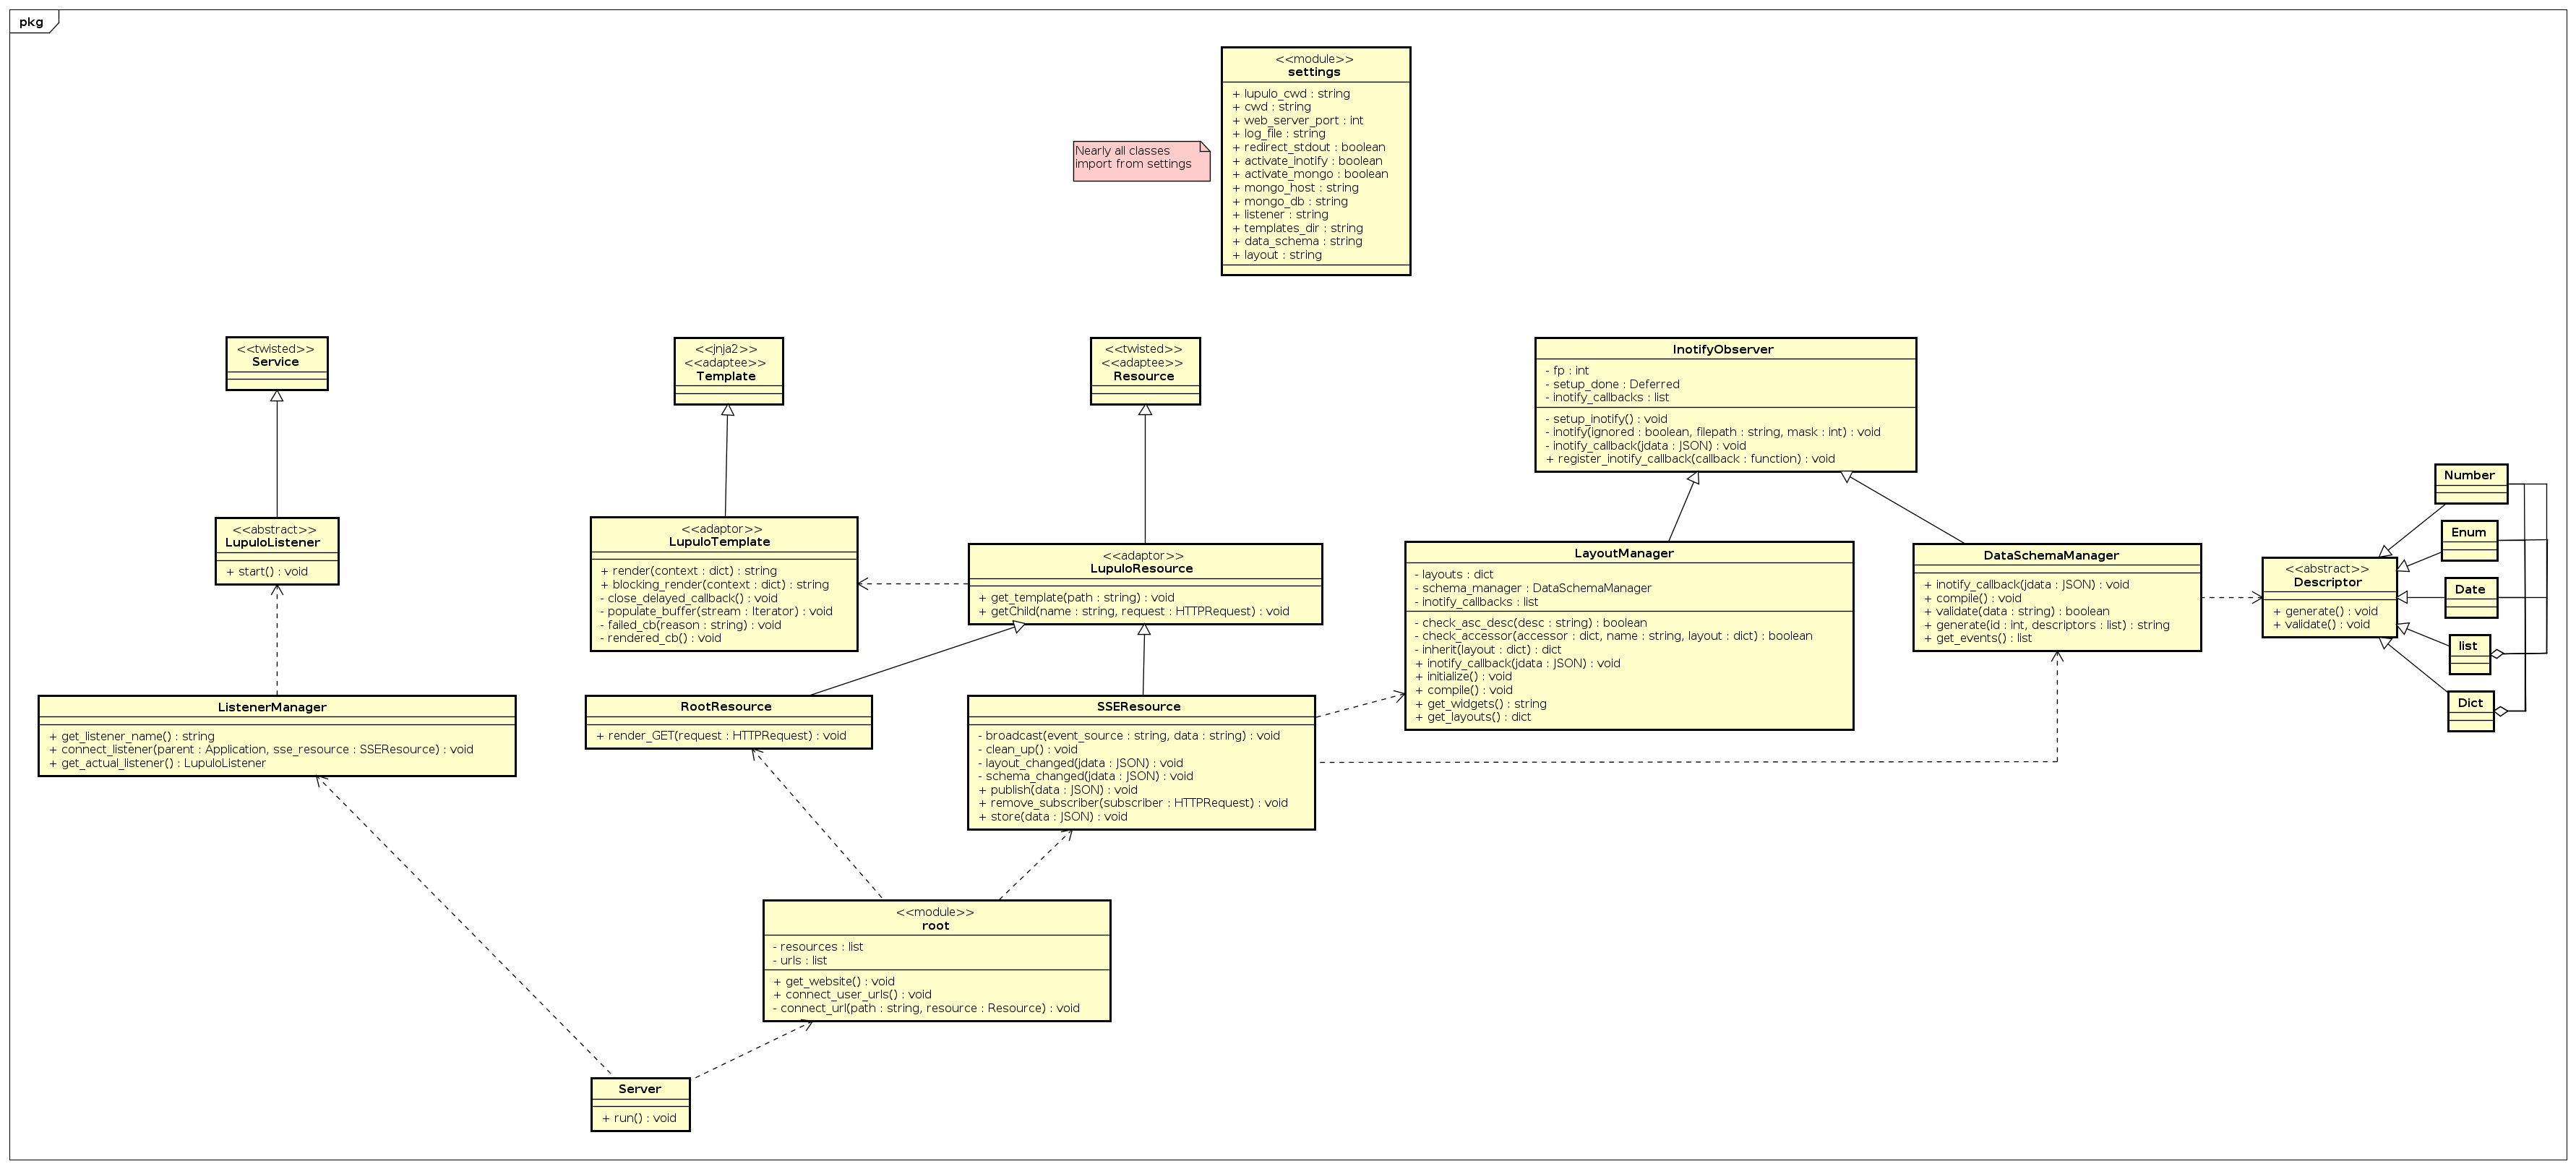
\includegraphics[height=0.8\textheight]{classes}
                    \caption{Classes diagram for the backend}
                \end{figure}
            \end{landscape}
            \restoregeometry

            The frontend is made of the following components:

            \begin{itemize}
                \item Controller for the events sent by the backend.
                \item Widget that renders information sent from the backend.
                \item Accessors abstraction.
            \end{itemize}

            \begin{figure}[h]
                \centering
                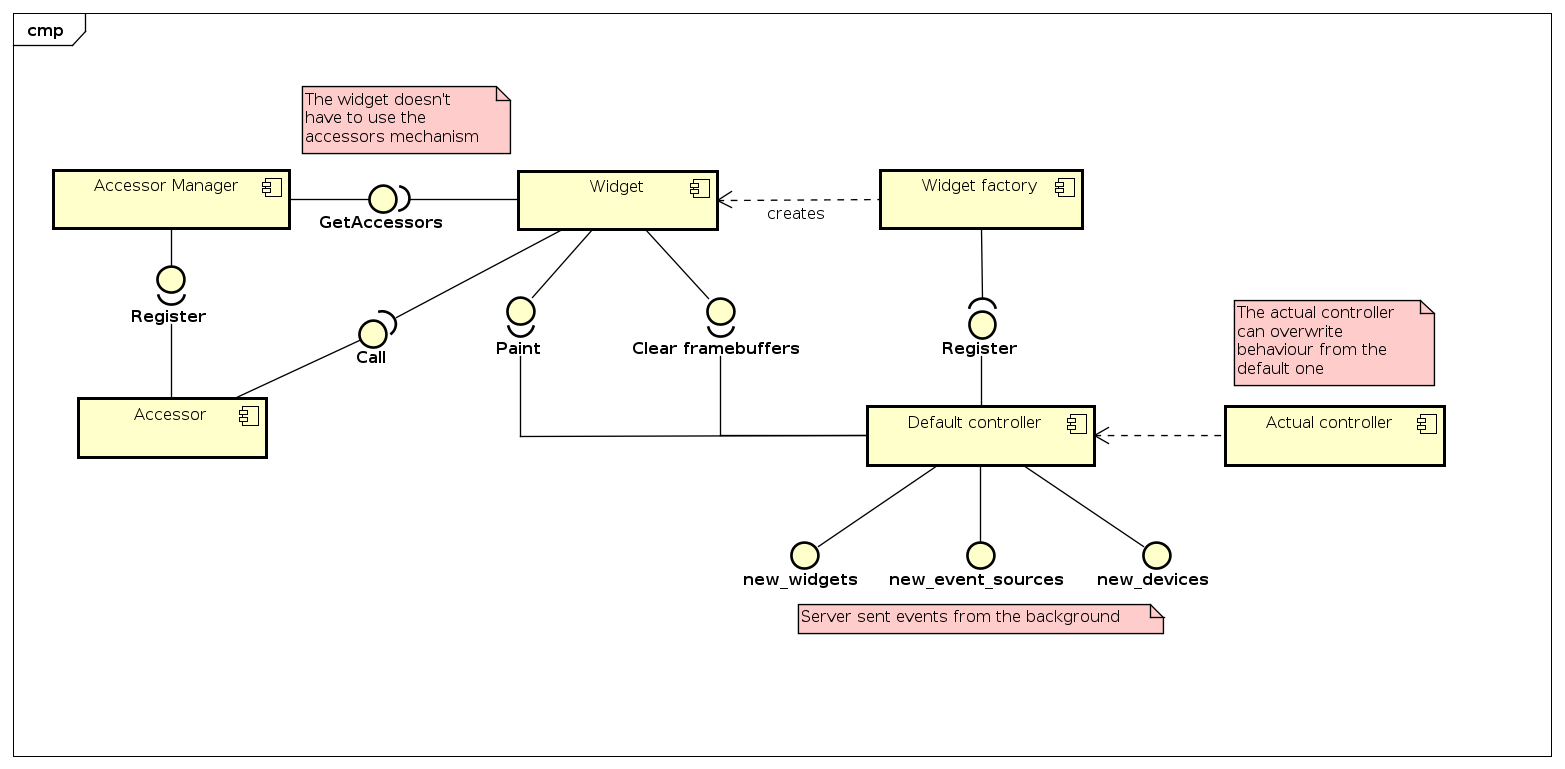
\includegraphics[width=\textwidth]{frontend}
                \caption{Main components for the frontend}
            \end{figure}

            The usual deployment of the project involves several hosts which run
            the backend, the optional store mechanism and the browser with the
            frontend loaded on it as can be seen in the following diagram.

            \begin{figure}[H]
                \centering
                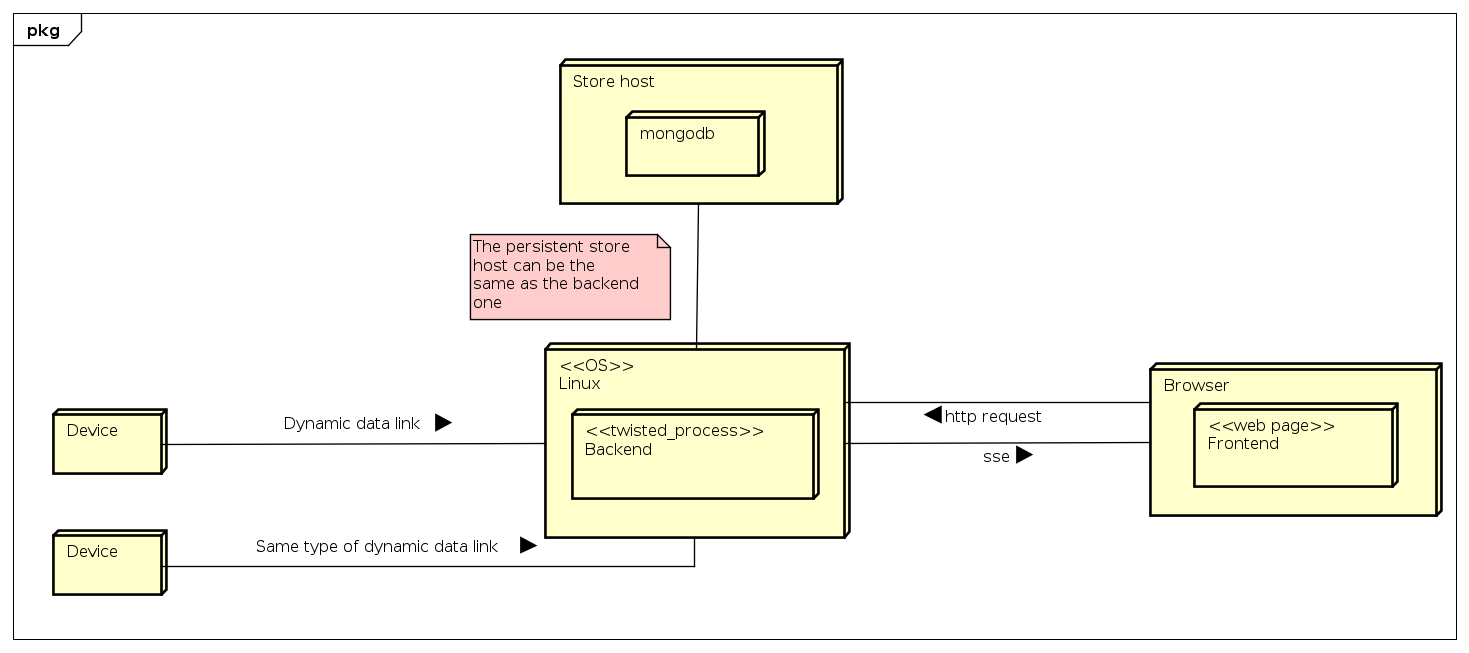
\includegraphics[width=\textwidth]{deployment}
                \caption{General deployment diagram}
            \end{figure}

        \subsection{Dynamic structure}
            Once the main structure of the project has been described, I'll
            explain the interactions of the software with several sequence
            diagrams that cover the main stages of lupulo once it has been
            started.

            \newgeometry{left=0.5cm, top=0.5cm, bottom=0.5cm}
            \thispagestyle{empty}
            \begin{landscape}
                \begin{figure}[h]
                    \centering
                    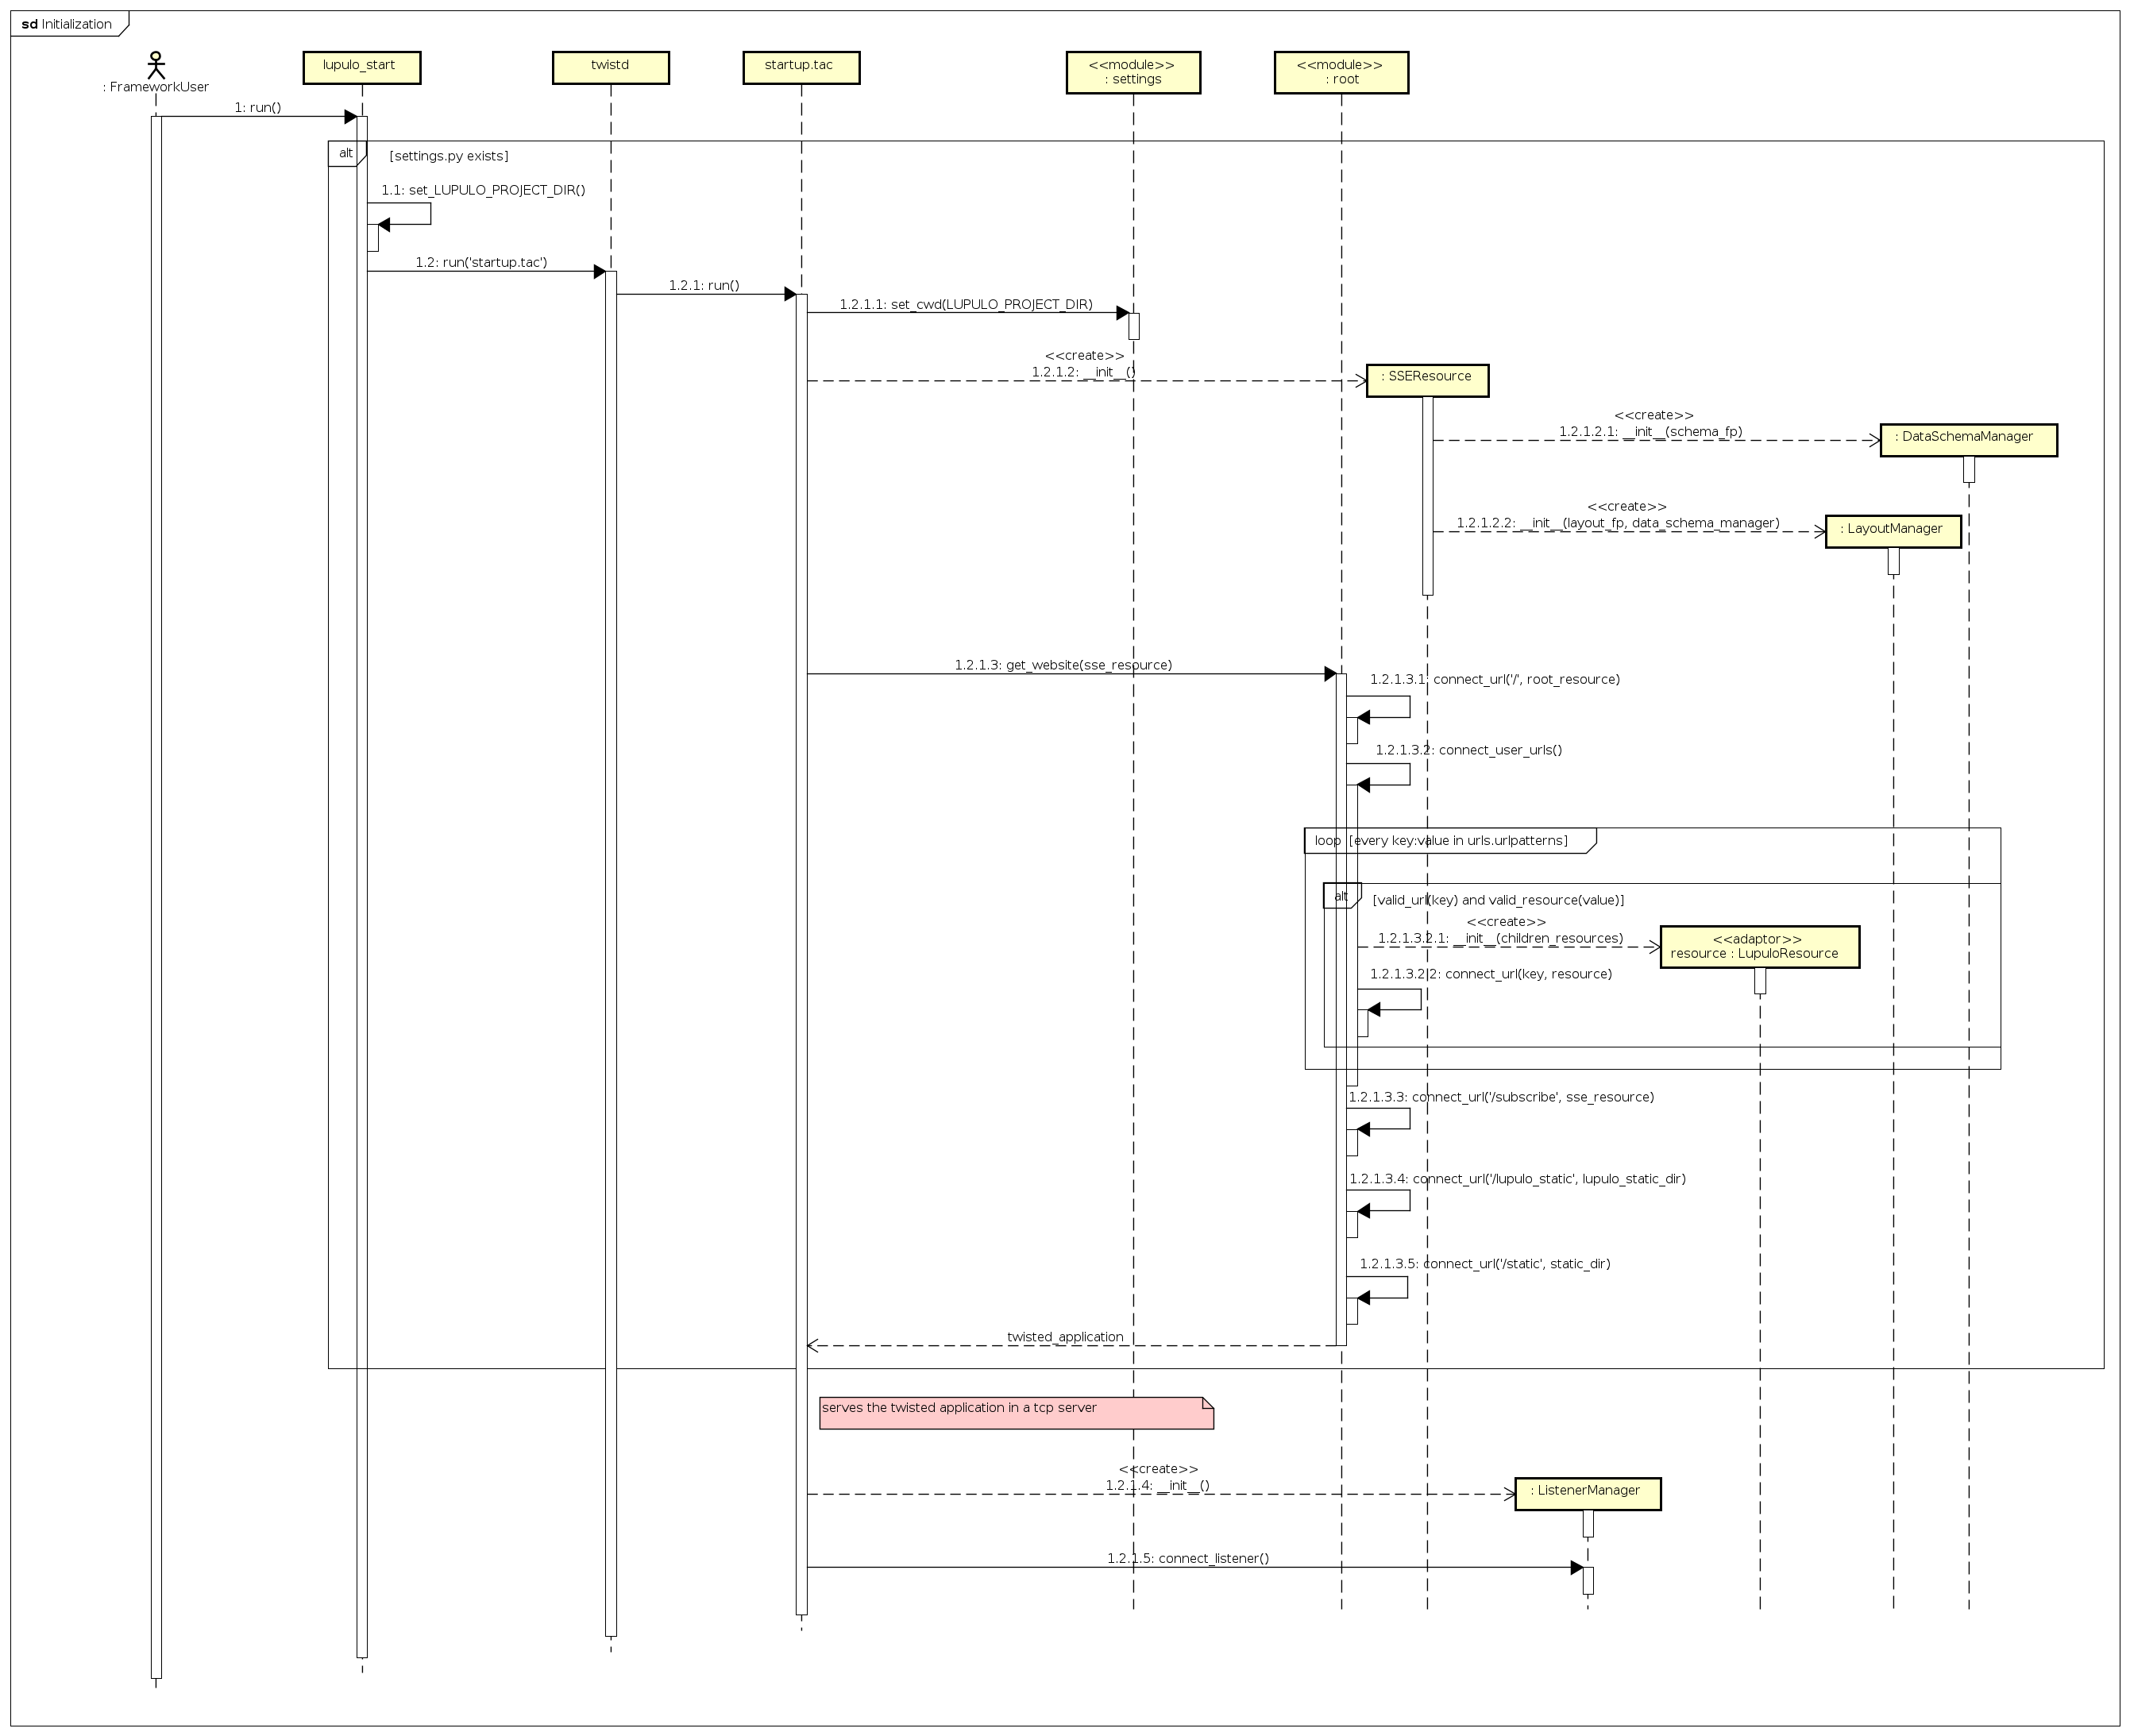
\includegraphics[height=1.1\textheight]{initialization}
                    \caption{Initialization of the backend}
                \end{figure}
            \end{landscape}
            \restoregeometry

            \newgeometry{left=0.5cm, top=0.5cm, bottom=0.5cm}
            \thispagestyle{empty}
                \begin{figure}[h]
                    \centering
                    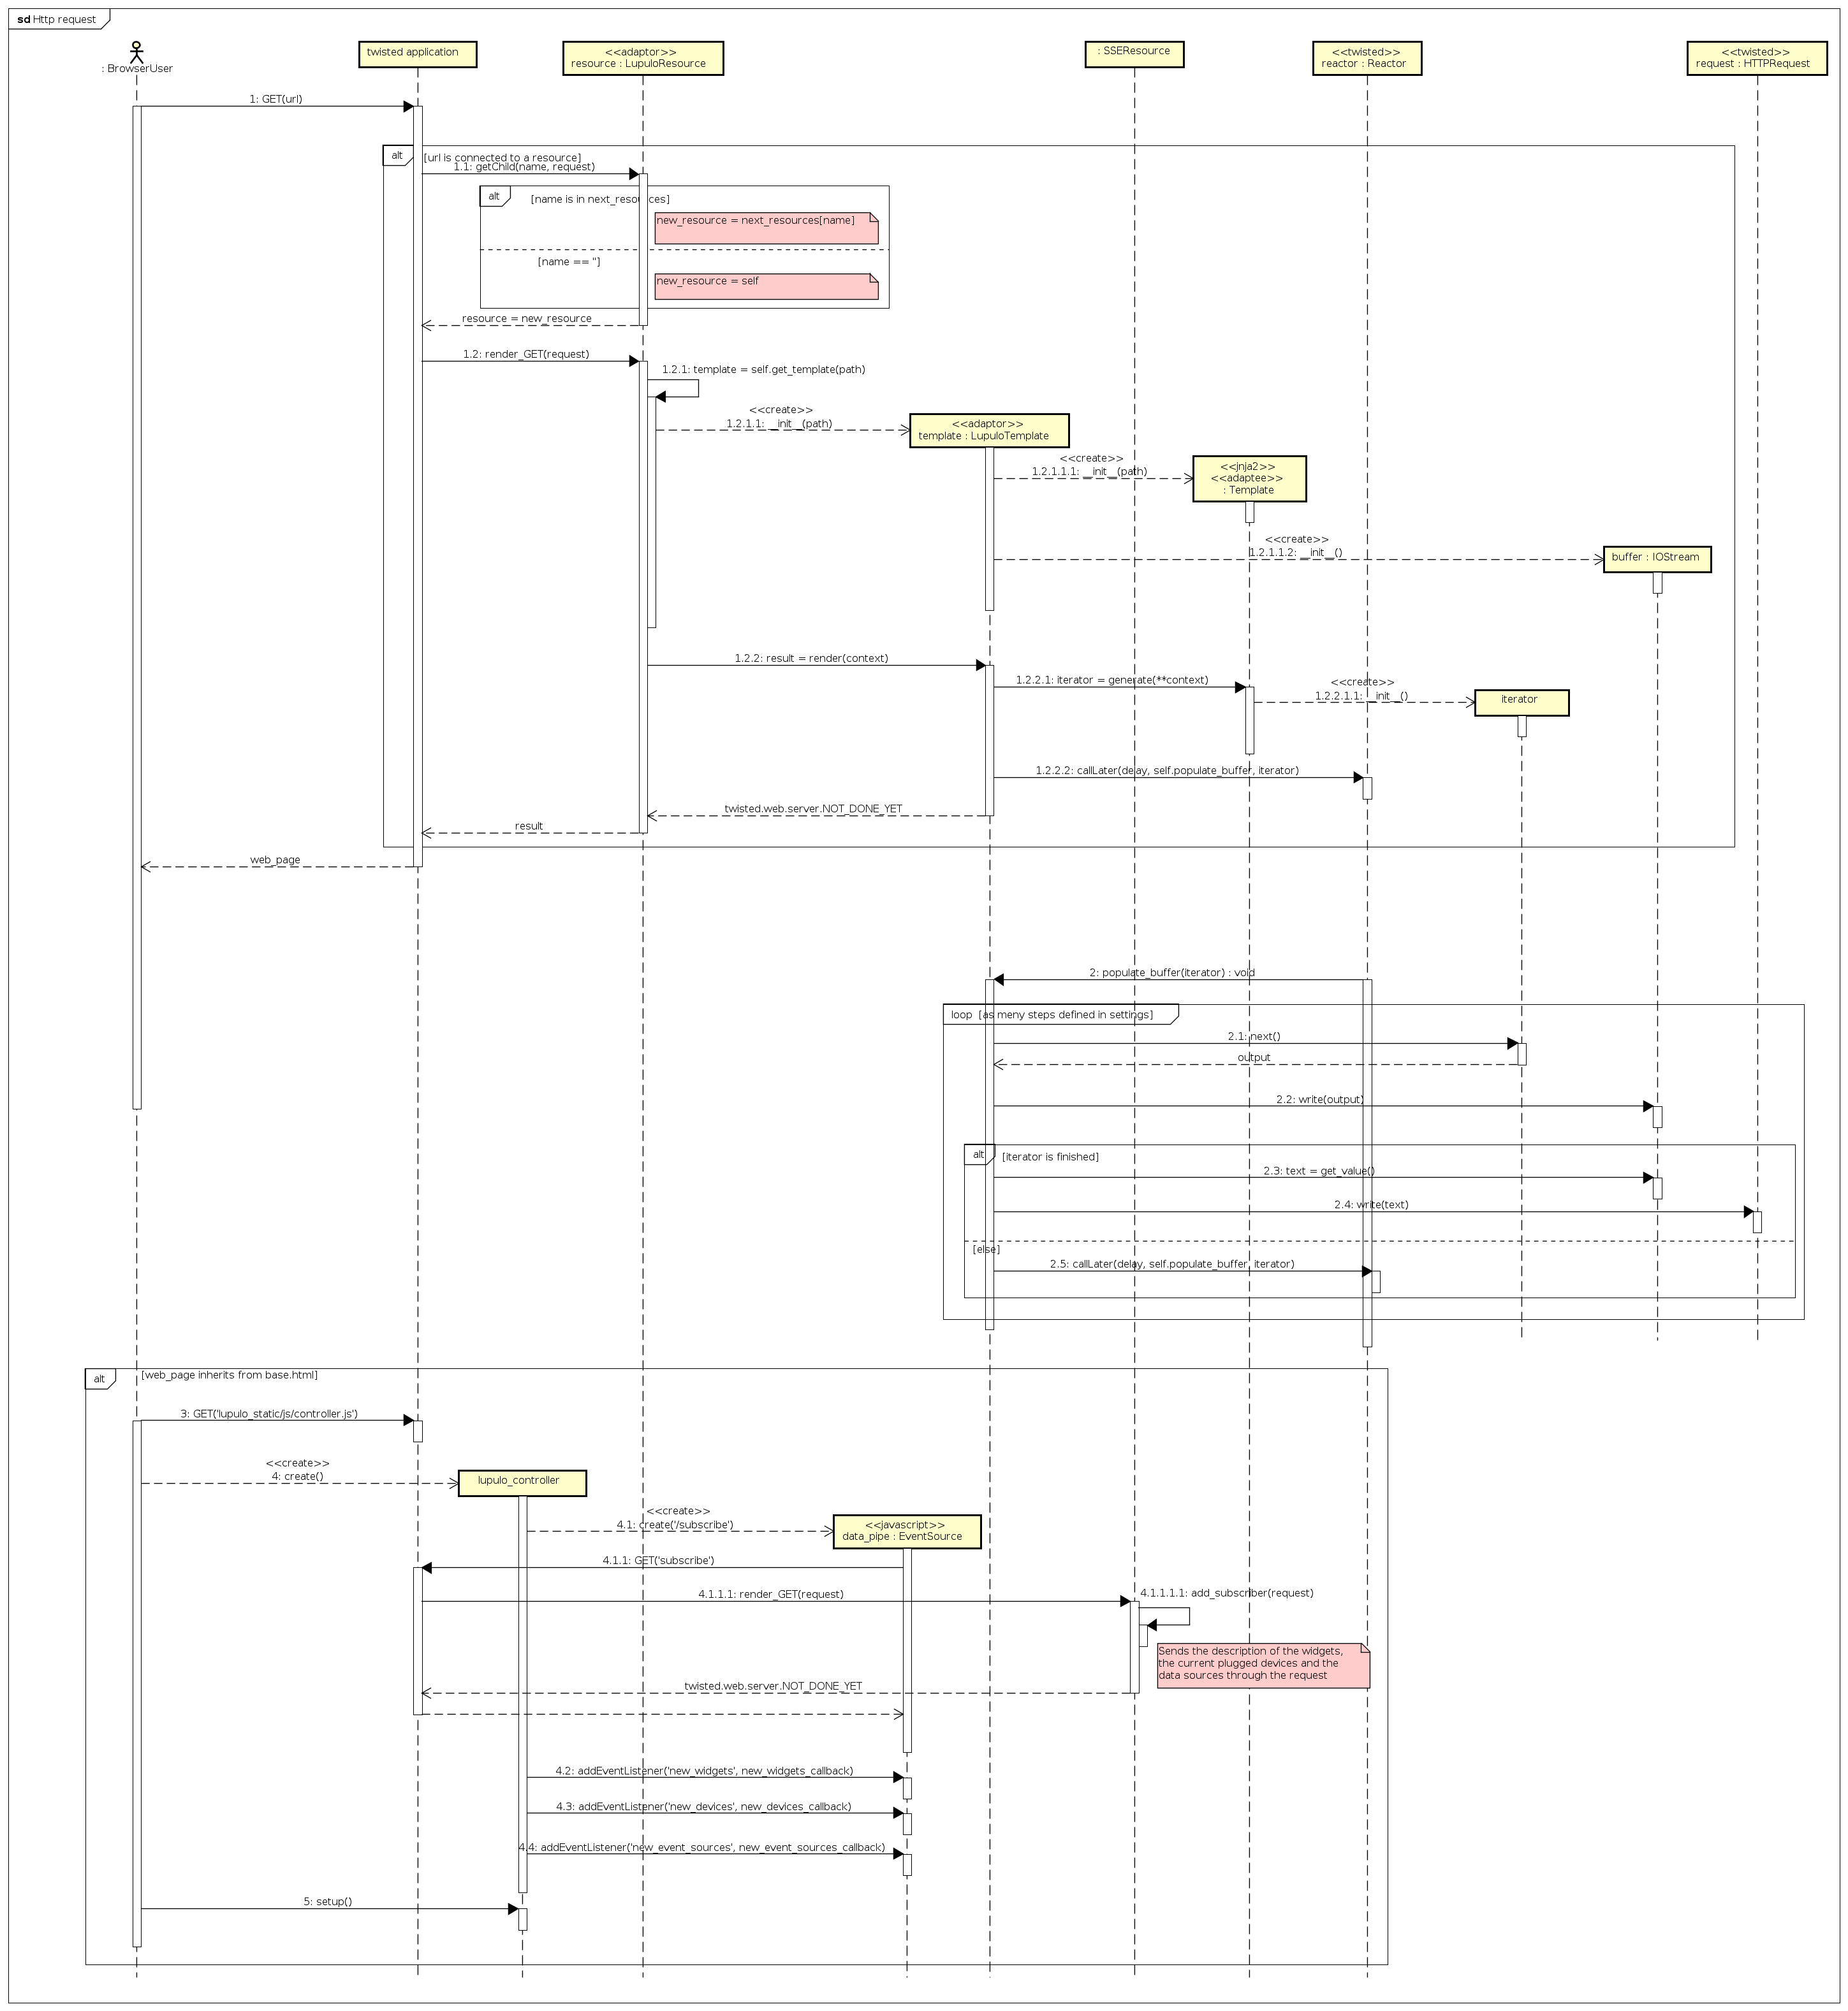
\includegraphics[width=1.15\textwidth]{http_request}
                    \caption{Http request from a browser asking for a web page
                    derived from base.html}
                \end{figure}
            \restoregeometry

            \newgeometry{left=0.5cm, top=0.5cm, bottom=0.5cm}
            \thispagestyle{empty}
            \begin{landscape}
                \begin{figure}[h]
                    \centering
                    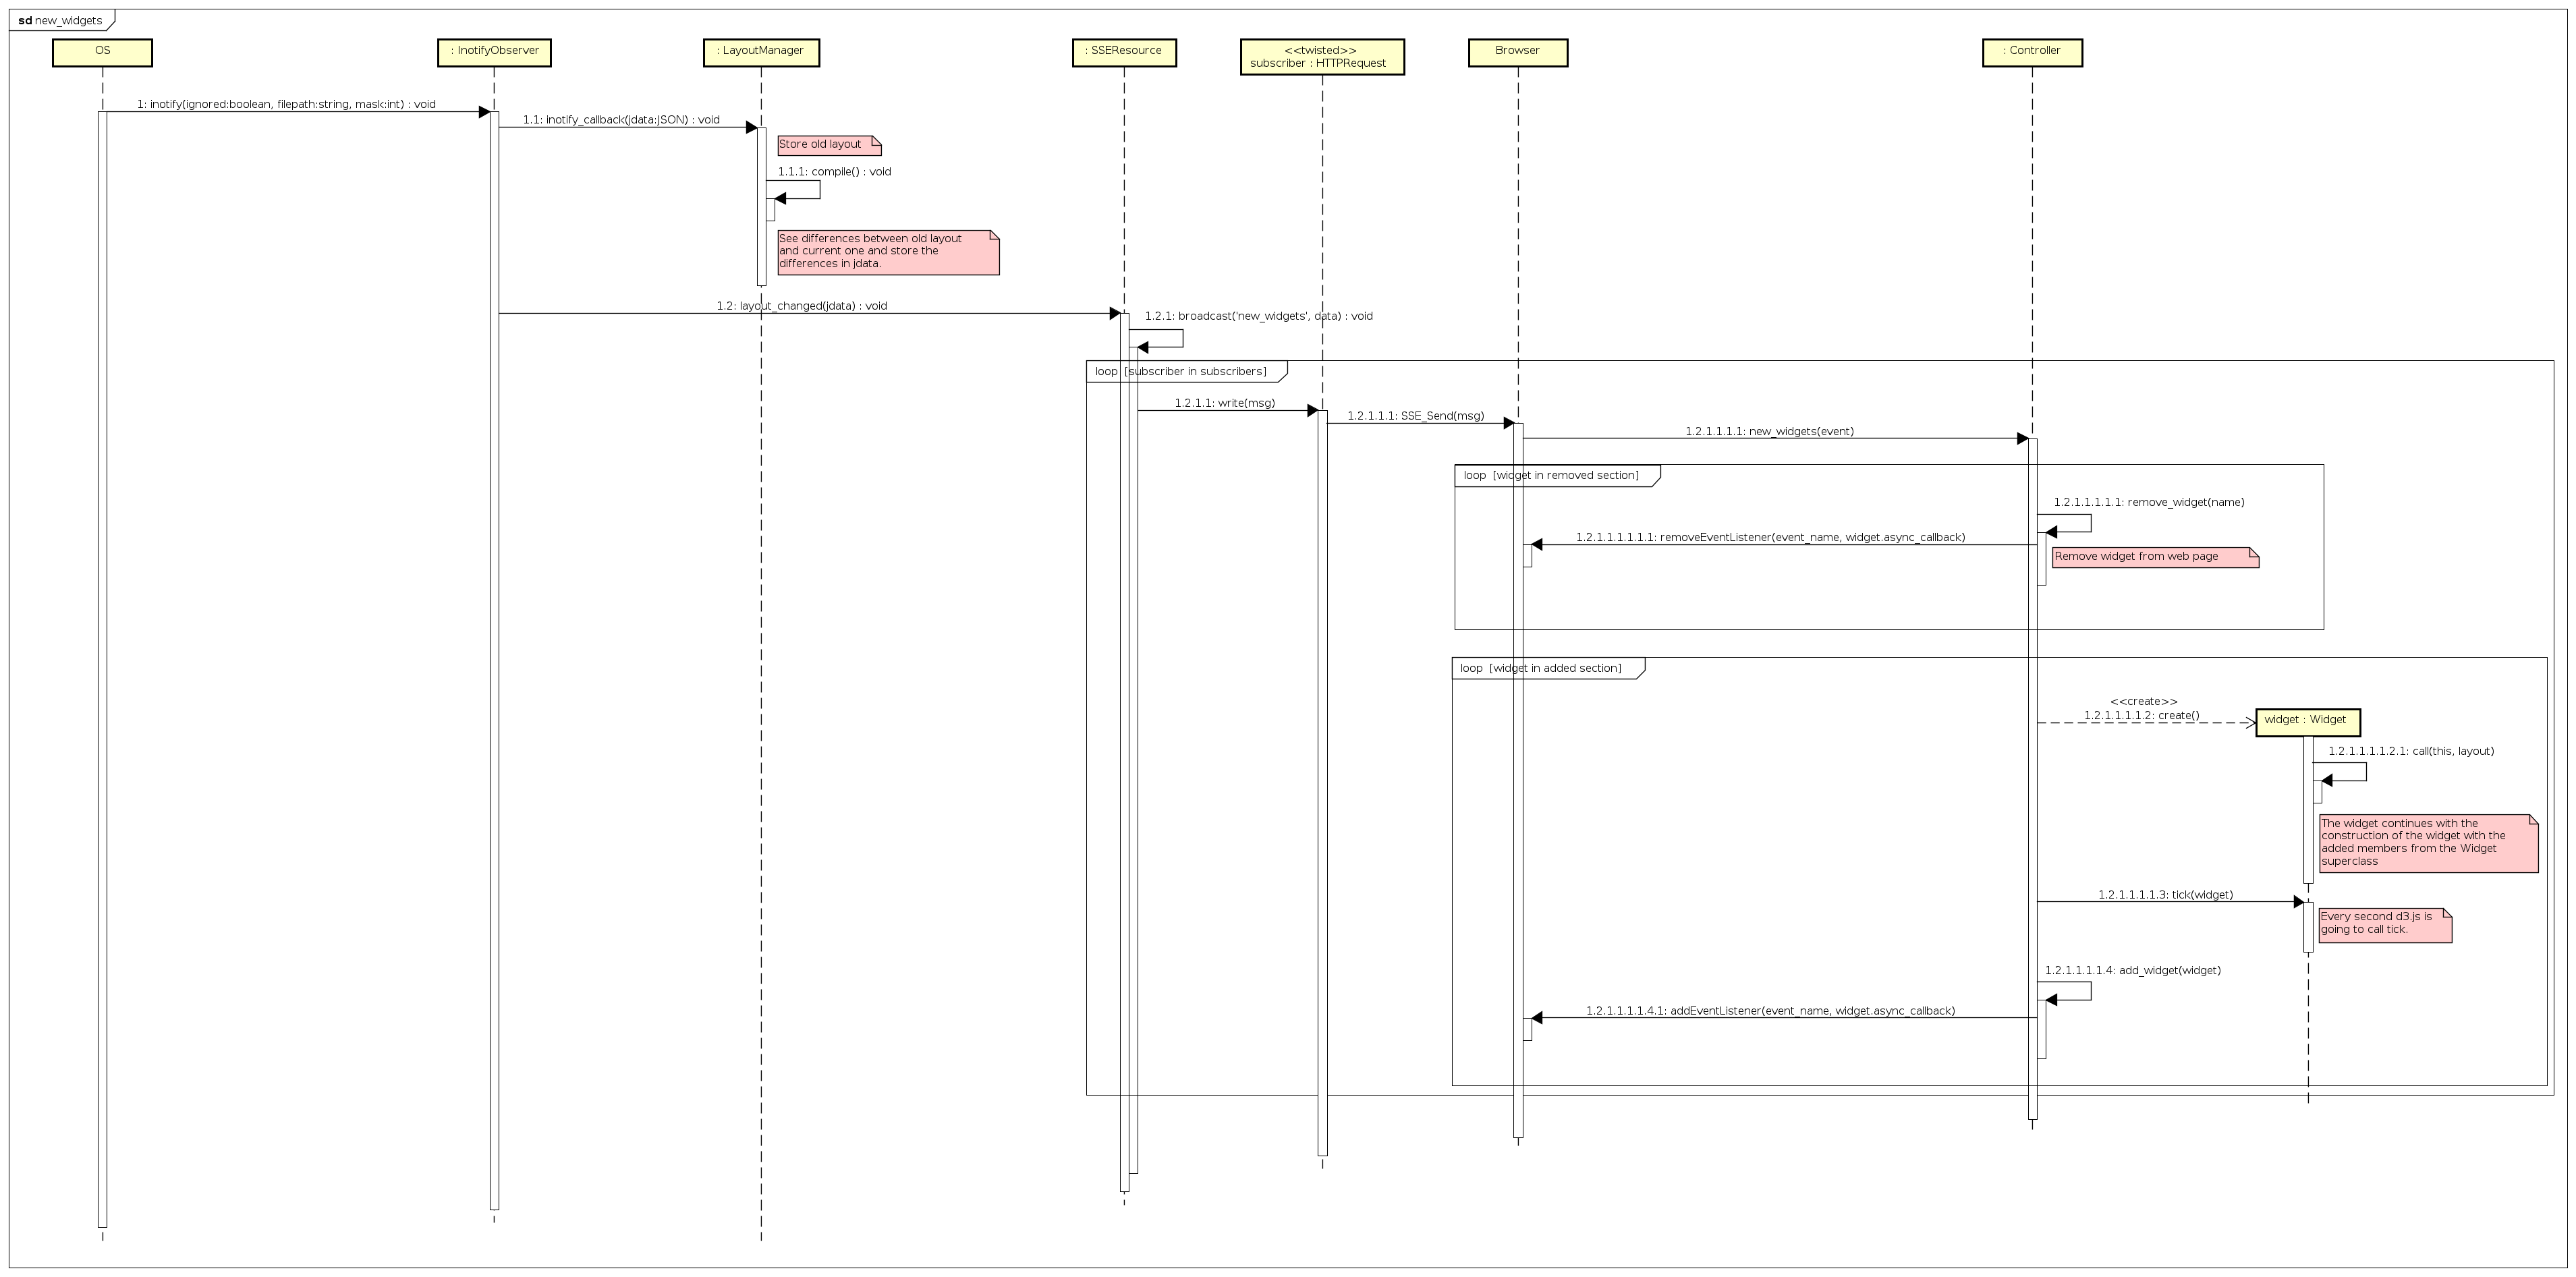
\includegraphics[height=0.75\textheight]{new_widgets}
                    \caption{Reception of a backend sse event, in particular
                    new\_widgets}
                \end{figure}
            \end{landscape}
            \restoregeometry

            \newgeometry{left=0.5cm, top=0.5cm, bottom=0.5cm}
            \thispagestyle{empty}
            \begin{landscape}
                \begin{figure}[h]
                    \centering
                    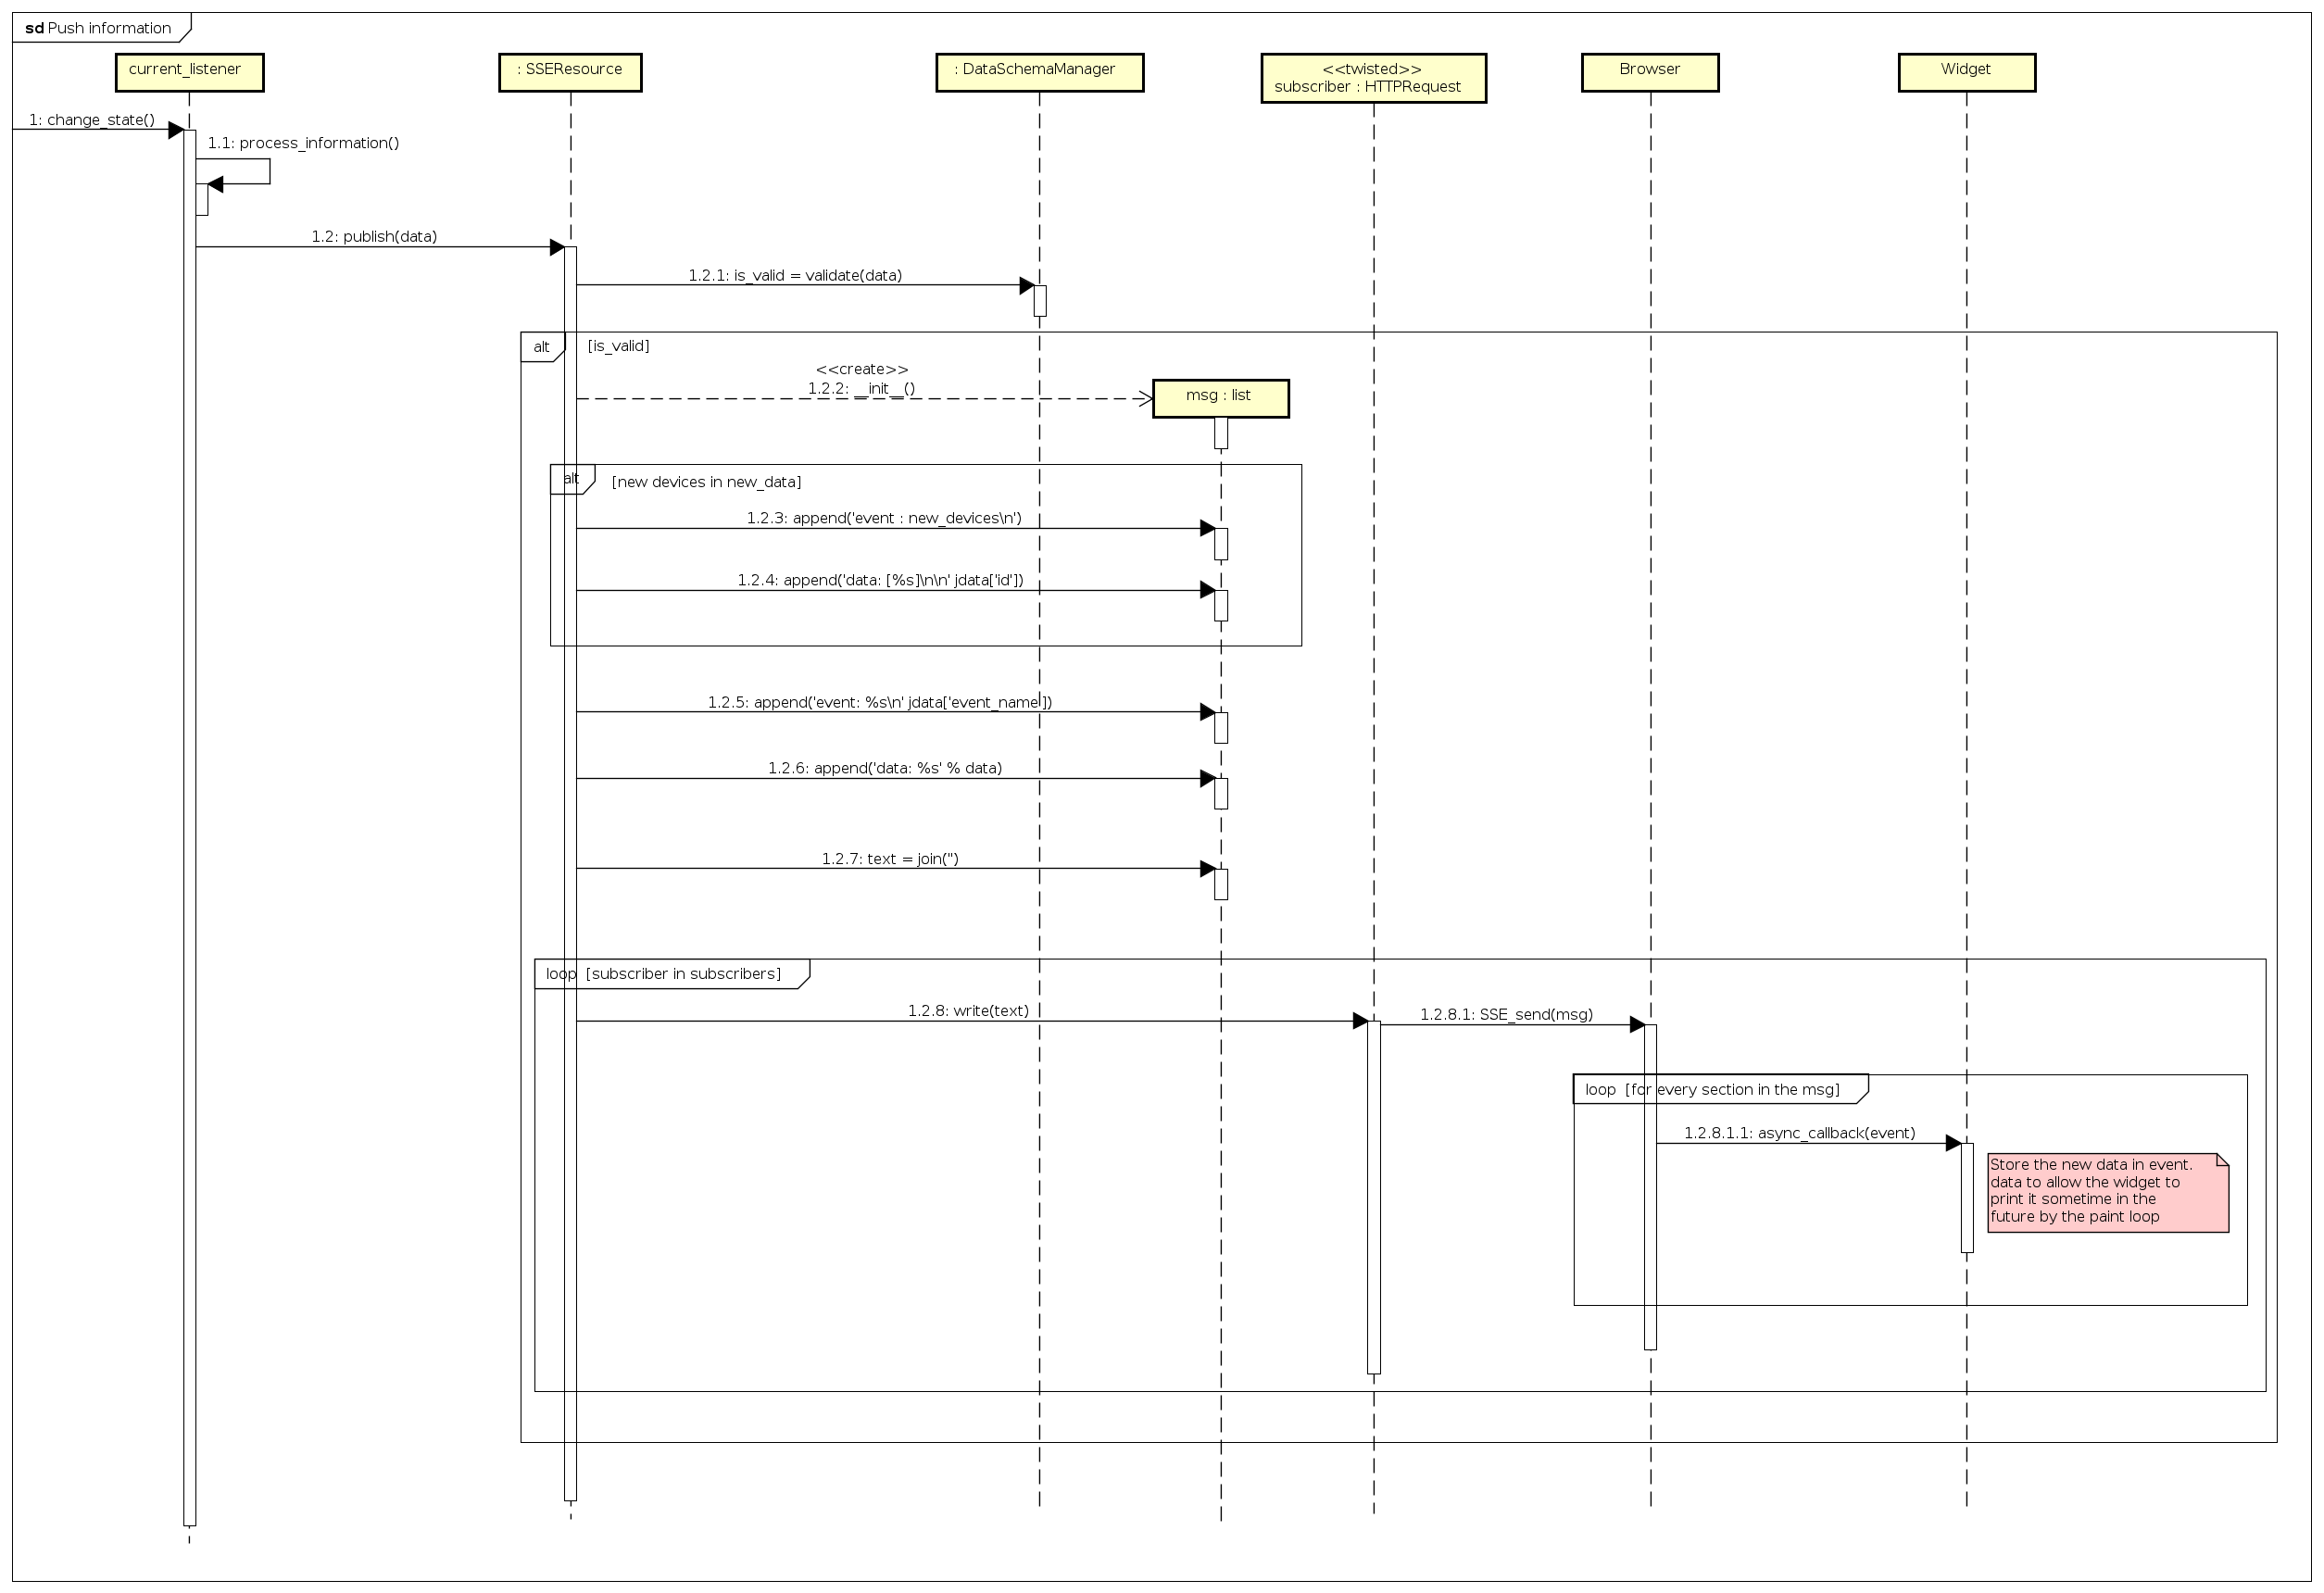
\includegraphics[height=\textheight]{push_information}
                    \caption{The backend pushes some information into the
                    frontend}
                \end{figure}
            \end{landscape}
            \restoregeometry

    \section{Methodology of work}
        I haven't followed strictly a methodology but a mix of them. Instead of
        following all the rules that a development methodology is made of, I
        have applied the principles it's base on to improve the quality of the
        software.
        
        That way, I have paid a lot of attention to the design of the
        architecture before its implementation was done to ensure that the
        structure of the software and the interactions between its different
        components was clean. I have also paid a lot of attention to the
        testing of the software to be able to change the architecture of the
        software without breaking everything in the process. Finally, the
        documentation is also very important for the project and I have invest a
        lot of time writing documentation for the potential users of the
        framework.

        Currently there are almost 100 tests in both the backend and the
        frontend that test every use case as a whole and in its smaller parts.

        Similarly, currently there are about 30 pages of documentation that
        cover every aspect of the framework in a detailed way to allow
        programmers an easy understanding without the need to read the source
        code. To allow people to contribute to the project, the source code is
        also commented to allow its easy understanding.

        I have followed the pep8 style guide in all my source code to ensure
        its cleanness, checking it periodically with an automated script.

        During the entire development of my final project I've been using git
        as a version control system for my source code putting special effort on
        branch management of the repository to allow an easy release and build
        management. The project is currently uploaded to pip with every major
        release uploaded to pip as long as it's possible.

        I have also used Redmine to report issues related to the software and
        also to have a record of how the project was evolving.

    \section{Work to do}
        There are several improvements to be done in the framework. The first
        one is to expand the number of listeners and widgets available at
        install time in the framework.

        The documentation should also include a tutorial to build a real time
        web page with the basic abstractions described above.

        The listeners abstraction could also be refactored to allow more than
        one type of listener to push information to the backend.

        The frontend could also be refactored in order to allow the use of html5
        canvas objects.

        More granularity in the paint loop should be provided to avoid different
        widget types to be called at different times.

    \section{Conclussions}
\end{document}
